\documentclass[11pt, a4paper]{report}
\usepackage[utf8]{inputenc}
\usepackage{pgfplots}

\usepackage[top=2cm, bottom=2.3cm, left=2cm, right=2cm]{geometry}

\title{Graficos das geracoes do NSGA2}
\author{Douglas Nunes de Oliveira}
\date{November 2021}


\begin{document}
    \begin{center}
        \textbf{Utilizando o NSGA2 para o problema de Schaffer modificado.}
        
        \textbf{Gráficos do espaço dos objetivos nas gerações ``1, 10, 50, 100 e 1000''}
        
        
    \end{center}
    

    \begin{center}
    \textbf{Geração 1}
\end{center}

\begin{figure}[h]
    \centering
    \label{fig:geracao01}
    
    \begin{tabular}{rl}
        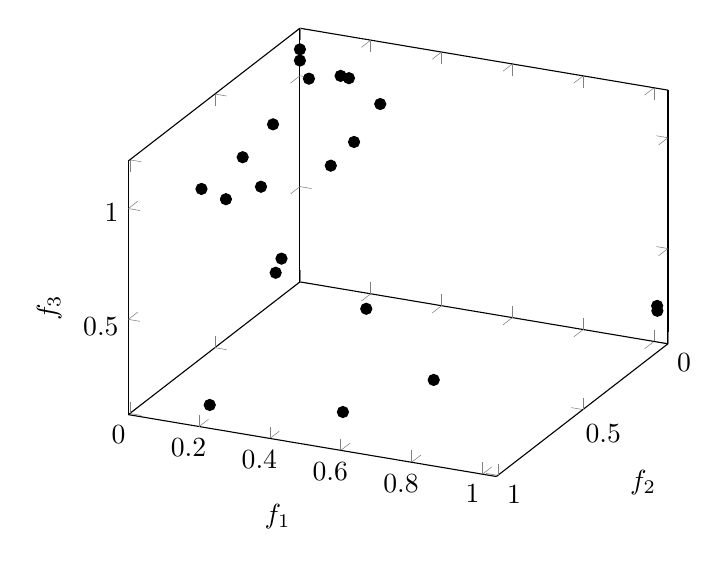
\begin{tikzpicture}[scale=1.0]
        	\begin{axis}[xlabel=$f_2$, ylabel=$f_1$, zlabel=$f_3$, view/h=115]
    			
    			\addplot3[only marks] coordinates {
            		(0.898985, 0.553341, 0.165563) (1.008660, 0.229953, 0.175532) (0.062171, 1.039330, 0.255872) (0.000000, 0.000000, 1.068948) (0.000000, 0.000000, 1.119406) (0.813499, 0.578235, 0.587300) (0.055647, 1.035543, 0.273132) (0.709822, 0.718883, 0.242456) (0.776314, 0.304513, 0.654200) (0.586016, 0.072568, 0.810780) (0.694715, 0.281731, 0.663309) (0.263698, 0.279511, 0.933176) (0.523794, 0.141747, 0.848635) (0.095871, 0.071497, 1.063344) (0.378926, 0.269237, 0.891967) (0.625020, 0.022316, 0.866778) (0.022923, 0.149424, 1.043225) (0.435767, 0.047729, 0.904337) (0.295924, 0.066268, 0.974661) (0.023673, 0.126287, 1.047775) (0.047674, 0.249717, 0.968201) 


        		};
        	\end{axis}
	    \end{tikzpicture}
	    &
	    \begin{tikzpicture}[scale=1.0]
        	\begin{axis}[xlabel=$f_2$, ylabel=$f_1$, zlabel=$f_3$, view={45}{0}]
    			
    			\addplot3[only marks] coordinates {
            		(0.198659,1.402927,0.030436)(0.243016,1.009920,0.490406)(0.965942,0.316067,0.944104)(0.926777,1.057248,0.066572)(0.755361,1.454336,0.018711)(1.099215,0.001117,0.701296)(0.930406,0.386454,0.145874)(0.363359,0.141019,1.073644)(0.005555,0.002258,1.133576)(1.244191,0.475865,0.000000)(0.055722,1.206260,0.087339)(0.122153,0.960673,0.791197)(1.197703,0.000000,0.012183)(0.338440,0.645361,1.002919)(1.231961,0.176431,0.126477)(0.842002,1.466963,0.128832)(1.400163,0.069214,0.140365)(0.050612,0.297072,1.183874)(0.177113,0.032273,1.369730)(0.096804,0.169118,1.443461)(1.185475,0.441860,0.309690) 

        		};
        	\end{axis}
	    \end{tikzpicture}
	\end{tabular}
    
\end{figure}


    \hrulefill
    \begin{center}
    \textbf{Geração 10}
\end{center}

\begin{figure}[h]
    \centering
    \label{fig:geracaoXX}
    
    \begin{tikzpicture}[scale=1.4]
        \begin{axis}[enlargelimits=false]
            \addplot [] coordinates {
                (0.000000,4.000000) (0.010000,3.610000) (0.040000,3.240000) (0.090000,2.890000) (0.160000,2.560000) (0.250000,2.250000) (0.360000,1.960000) (0.490000,1.690000) (0.640000,1.440000) (0.810000,1.210000) (1.000000,1.000000) (1.210000,0.810000) (1.440000,0.640000) (1.690000,0.490000) (1.960000,0.360000) (2.250000,0.250000) (2.560000,0.160000) (2.890000,0.090000) (3.240000,0.040000) (3.610000,0.010000) (4.000000,0.000000) 
            };
            
            \addplot [only marks] coordinates {
                (9.765582,16.939883)(9.924204,17.003386)(10.091199,17.110039)(10.211898,17.205926)(10.337007,17.555696)(12.514860,17.518859)(13.126414,18.337417)(17.804570,20.690929)(70.410450,56.563290)(71.896435,90.028819)(72.099991,90.135653)(72.732258,90.743713)(72.980565,91.249132)(73.640637,91.289447)(73.857270,91.995217)(75.358388,92.246202)(75.811555,94.296171)(76.248114,94.129894)(76.362091,94.174254)(76.250749,94.632550) 
            };
        \end{axis}
    \end{tikzpicture}
\end{figure}

    \newpage

    \begin{center}
    \textbf{Geração 50}
\end{center}

\begin{figure}[h]
    \centering
    \label{fig:geracaoXX}
    
    \begin{tikzpicture}[scale=1.4]
        \begin{axis}[enlargelimits=false]
            \addplot [] coordinates {
                (0.000000,4.000000) (0.010000,3.610000) (0.040000,3.240000) (0.090000,2.890000) (0.160000,2.560000) (0.250000,2.250000) (0.360000,1.960000) (0.490000,1.690000) (0.640000,1.440000) (0.810000,1.210000) (1.000000,1.000000) (1.210000,0.810000) (1.440000,0.640000) (1.690000,0.490000) (1.960000,0.360000) (2.250000,0.250000) (2.560000,0.160000) (2.890000,0.090000) (3.240000,0.040000) (3.610000,0.010000) (4.000000,0.000000) 
            };
            
            \addplot [only marks] coordinates {
                (7.079039,9.893604)(6.998996,10.667901)(7.153247,10.267265)(7.675170,10.023482)(7.176644,10.167450)(7.684816,10.057420)(7.337534,10.589789)(7.258915,11.093974)(7.387049,10.466614)(7.385134,10.873843)(7.421006,10.594347)(7.413217,11.198653)(7.536725,10.792519)(7.722630,10.658570)(7.437473,10.984634)(7.596418,10.718251)(7.577853,11.008782)(7.721938,10.867479)(8.215063,10.807069)(8.124915,10.913137)
            };
        \end{axis}
    \end{tikzpicture}
\end{figure}
    \hrulefill
    \begin{center}
    \textbf{Geração 100}
\end{center}

\begin{figure}[h]
    \centering
    \label{fig:geracao01}
    
    \begin{tabular}{rl}
        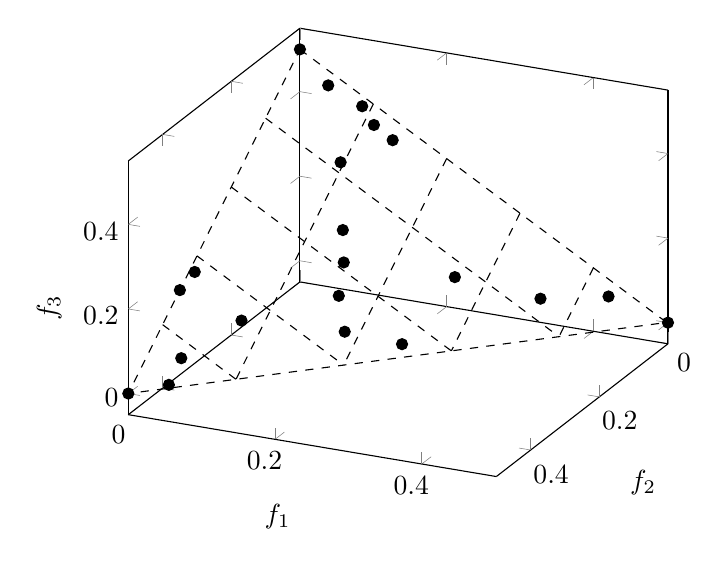
\begin{tikzpicture}[scale=1.0]
        	\begin{axis}[xlabel=$f_2$, ylabel=$f_1$, zlabel=$f_3$, view/h=115]
        		
    			\addplot3[style={dashed}]coordinates {
    			    (0., 0., 0.5) (0., 0.5, 0.) (0.5, 0., 0.) (0., 0., 0.5)
    			};
    			
    			\addplot3[style={dashed}]coordinates {(0., 0.1, 0.4) (0.4, 0.1, 0.)};
    			\addplot3[style={dashed}]coordinates {(0., 0.2, 0.3) (0.3, 0.2, 0.)};
    			\addplot3[style={dashed}]coordinates {(0., 0.3, 0.2) (0.2, 0.3, 0.)};
    			\addplot3[style={dashed}]coordinates {(0., 0.4, 0.1) (0.1, 0.4, 0.)};
    			
    			\addplot3[style={dashed}]coordinates {(0.4, 0., 0.1) (0.4, 0.1, 0.)};
    			\addplot3[style={dashed}]coordinates {(0.3, 0., 0.2) (0.3, 0.2, 0.)};
    			\addplot3[style={dashed}]coordinates {(0.2, 0., 0.3) (0.2, 0.3, 0.)};
    			\addplot3[style={dashed}]coordinates {(0.1, 0., 0.4) (0.1, 0.4, 0.)};
    			
    			\addplot3[only marks] coordinates {
            		(0.500000, 0.000000, 0.000000) (0.000000, 0.501703, 0.000000) (0.000000, 0.000000, 0.500000) (0.157649, 0.132235, 0.210208) (0.087593, 0.096445, 0.316043) (0.015851, 0.045971, 0.438178) (0.421486, 0.035456, 0.044608) (0.264481, 0.184805, 0.052188) (0.119914, 0.267315, 0.114612) (0.022538, 0.111409, 0.367816) (0.019174, 0.429660, 0.052998) (0.318838, 0.005763, 0.175425) (0.074387, 0.362737, 0.062880) (0.011178, 0.090107, 0.398780) (0.231305, 0.161214, 0.109347) (0.191210, 0.149214, 0.159667) (0.349778, 0.000000, 0.150250) (0.459634, 0.036409, 0.005755) (0.334294, 0.076760, 0.090826) (0.232486, 0.247968, 0.021100) (0.024000, 0.137638, 0.340430) 

        		};
        	\end{axis}
	    \end{tikzpicture}
	    &
	    \begin{tikzpicture}[scale=1.0]
        	\begin{axis}[xlabel=$f_2$, ylabel=$f_1$, zlabel=$f_3$, view={45}{0}]
        		
    			\addplot3[style={dashed}]coordinates {
    			    (0., 0., 0.5) (0., 0.5, 0.) (0.5, 0., 0.) (0., 0., 0.5)
    			};
    			
    			\addplot3[only marks] coordinates {
            		(17.814138,0.000000,0.000000)(0.000000,17.643105,0.000000)(0.000000,0.000000,13.977723)(1.601047,10.251867,7.614543)(8.135195,5.670870,2.084032)(1.035720,4.965857,12.009724)(4.364600,12.359378,0.631340)(1.928931,8.790747,6.922857)(6.735992,0.000000,10.180065)(11.212573,0.832881,5.485430)(10.144734,0.000000,6.517945)(15.368517,0.000000,2.597986)(2.658333,6.603699,4.139209)(14.381035,2.091973,0.851876)(0.602773,11.579934,1.417001)(5.429664,5.099744,3.936790)(6.220722,1.214467,10.351246)(3.204461,14.638293,0.000000)(11.832449,0.000000,4.804166)(0.180017,0.101508,13.393921)(2.804775,14.865582,0.000000) 

        		};
        	\end{axis}
	    \end{tikzpicture}
	\end{tabular}
    
\end{figure}


    
    \newpage
    \begin{center}
    \textbf{Geração 1000}
\end{center}

\begin{figure}[h]
    \centering
    \label{fig:geracao01}
    
    \begin{tabular}{rl}
        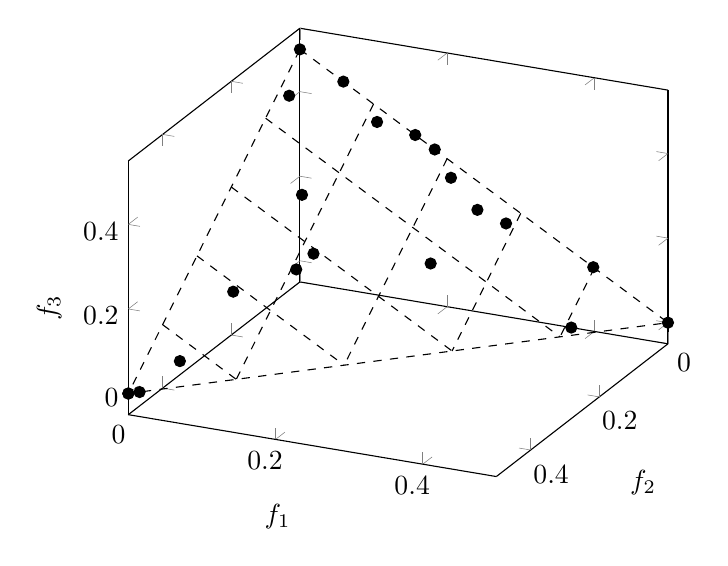
\begin{tikzpicture}[scale=1.0]
        	\begin{axis}[xlabel=$f_2$, ylabel=$f_1$, zlabel=$f_3$, view/h=115]
        		
    			\addplot3[style={dashed}]coordinates {
    			    (0., 0., 0.5) (0., 0.5, 0.) (0.5, 0., 0.) (0., 0., 0.5)
    			};
    			
    			\addplot3[style={dashed}]coordinates {(0., 0.1, 0.4) (0.4, 0.1, 0.)};
    			\addplot3[style={dashed}]coordinates {(0., 0.2, 0.3) (0.3, 0.2, 0.)};
    			\addplot3[style={dashed}]coordinates {(0., 0.3, 0.2) (0.2, 0.3, 0.)};
    			\addplot3[style={dashed}]coordinates {(0., 0.4, 0.1) (0.1, 0.4, 0.)};
    			
    			\addplot3[style={dashed}]coordinates {(0.4, 0., 0.1) (0.4, 0.1, 0.)};
    			\addplot3[style={dashed}]coordinates {(0.3, 0., 0.2) (0.3, 0.2, 0.)};
    			\addplot3[style={dashed}]coordinates {(0.2, 0., 0.3) (0.2, 0.3, 0.)};
    			\addplot3[style={dashed}]coordinates {(0.1, 0., 0.4) (0.1, 0.4, 0.)};
    			
    			\addplot3[only marks] coordinates {
            		(0.500000, 0.000000, 0.000000) (0.500000, 0.000000, 0.000000) (0.000000, 0.500000, 0.000000) (0.000000, 0.000000, 0.500000) (0.022317, 0.290411, 0.187272) (0.000000, 0.398503, 0.101497) (0.309423, 0.053651, 0.136926) (0.152593, 0.073964, 0.273443) (0.236225, 0.105143, 0.158632) (0.000000, 0.156647, 0.343353) (0.000000, 0.183146, 0.316854) (0.016253, 0.112373, 0.371374) (0.425035, 0.035095, 0.039870) (0.057607, 0.012249, 0.430144) (0.030429, 0.255305, 0.214266) (0.017226, 0.213245, 0.269528) (0.205948, 0.114458, 0.179594) (0.081295, 0.406565, 0.012140) (0.124109, 0.235478, 0.140413) (0.489575, 0.010425, 0.000000) (0.000000, 0.058984, 0.441016) 

        		};
        	\end{axis}
	    \end{tikzpicture}
	    &
	    \begin{tikzpicture}[scale=1.0]
        	\begin{axis}[xlabel=$f_2$, ylabel=$f_1$, zlabel=$f_3$, view={45}{0}]
        		
    			\addplot3[style={dashed}]coordinates {
    			    (0., 0., 0.5) (0., 0.5, 0.) (0.5, 0., 0.) (0., 0., 0.5)
    			};
    			
    			\addplot3[only marks] coordinates {
            		(13.026614,0.000000,0.000000)(0.000000,13.026614,0.000000)(0.000000,0.000000,13.026614)(6.607459,2.768464,3.650691)(8.858561,4.168053,0.000000)(4.775350,0.153626,8.097638)(0.038916,3.832737,9.154961)(2.465687,7.841465,2.719462)(0.389702,1.190070,11.446843)(0.019892,10.608245,2.398477)(11.740882,0.905432,0.380301)(10.612149,0.184901,2.229564)(6.328799,0.000000,6.697815)(4.073184,1.682148,7.271282)(1.709631,5.620078,5.696905)(1.920648,6.341865,4.764101)(0.678180,12.348434,0.000000)(0.770733,3.459635,8.796247)(2.439457,7.967100,2.620058)(7.657499,1.655864,3.713251)(3.378821,9.647794,0.000000)

        		};
        	\end{axis}
	    \end{tikzpicture}
	\end{tabular}
    
\end{figure}


    \hrulefill

\end{document}
